\begin{frame}
    \autotitle
    \begin{center}
        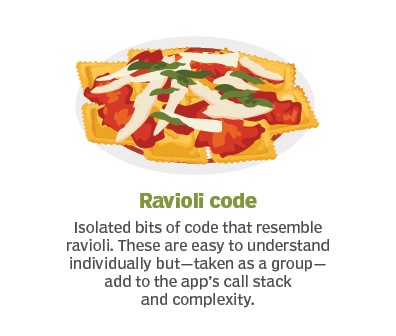
\includegraphics[scale=.5]{img/ravioli.png}
    \end{center}
\end{frame}

\begin{frame}
    \autotitle
    \begin{center}
        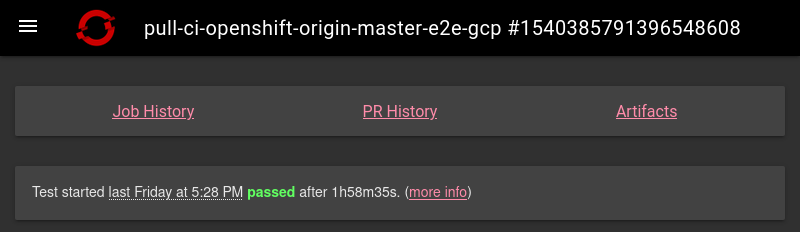
\includegraphics[width=\textwidth]{../ci-operator/img/job.png}
        \footnotesize
        \url{https://prow.ci.openshift.org/view/gs/origin-ci-test/pr-logs/pull/27275/pull-ci-openshift-origin-master-e2e-gcp/1540385791396548608}
    \end{center}
    \note{
        We will revisit today the example job we looked at in the last third of
        the previous presentation, now in much more detail.
    }
\end{frame}

\begin{frame}[fragile]
    \autotitle
    \tiny
    \url{https://gcsweb-ci.apps.ci.l2s4.p1.openshiftapps.com/gcs/origin-ci-test/pr-logs/pull/27275/pull-ci-openshift-origin-master-e2e-gcp/1540385791396548608/prowjob.json}*
    \footnotesize
    \begin{verbatim}
command:
- ci-operator
args:
- --gcs-upload-secret=/secrets/gcs/service-account.json
- --image-import-pull-secret=/etc/pull-secret/.dockerconfigjson
- --lease-server-credentials-file=/etc/boskos/credentials
- --report-credentials-file=/etc/report/credentials
- --secret-dir=/secrets/ci-pull-credentials
- --secret-dir=/usr/local/e2e-gcp-cluster-profile
- --target=e2e-gcp
    \end{verbatim}
    \vfill
    \small
    *\href{https://github.com/openshift/ci-docs/pull/266}{
        \textit{how-tos: document artifacts directory} \#266
        --- \texttt{openshift/ci-docs}
    }
    \note{
        As a reminder, this will (via \texttt{prowgen}) result in a
        \texttt{ProwJob} which will execute \texttt{ci-operator} targeting the
        single test name \texttt{e2e-gcp}, declared in its configuration file
        (obtained from the \texttt{configresolver}).
    }
\end{frame}

\begin{frame}
    \autotitle
    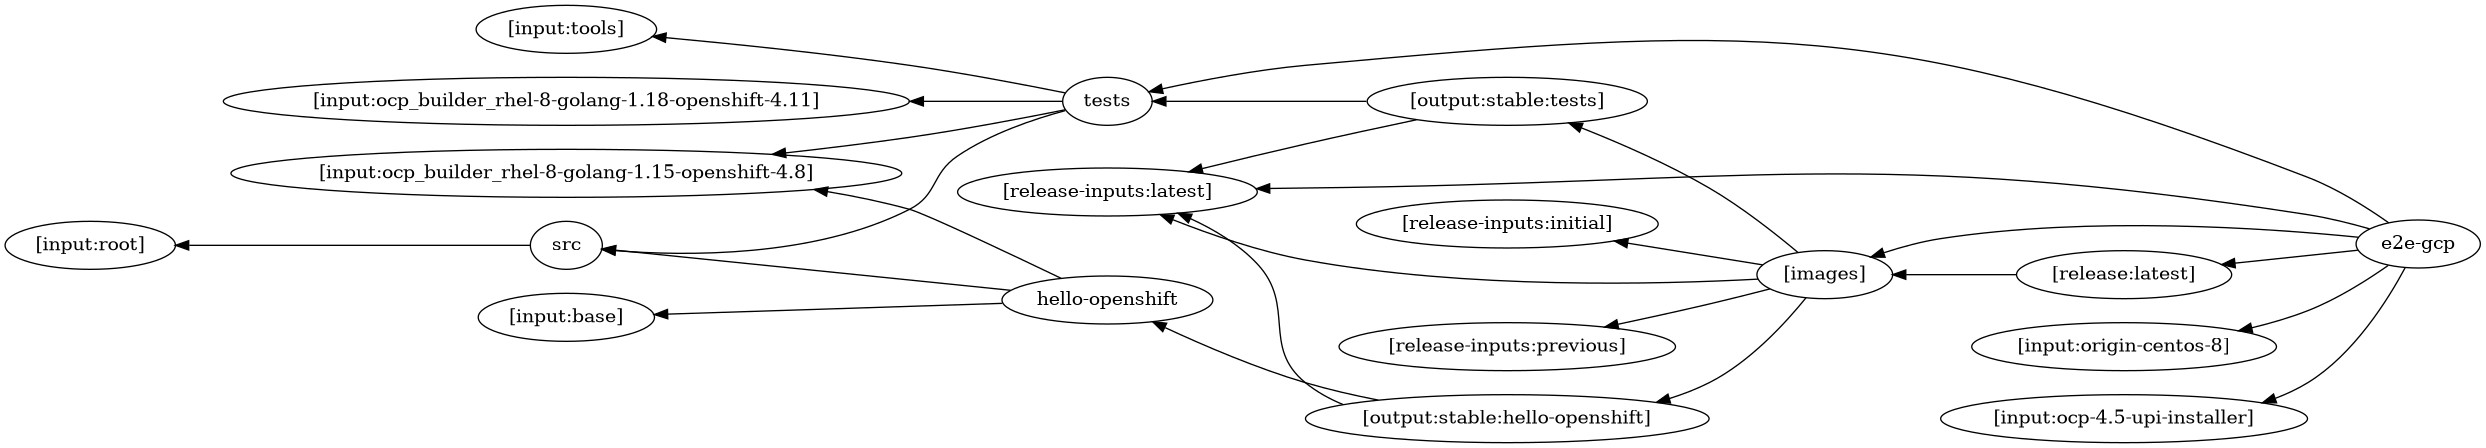
\includegraphics[width=\textwidth]{../ci-operator/img/graph_origin_gcp.jpg}
    \note{
        And this will be done by constructing and execting this step graph.  See
        the previous presentation for a reminder of how all of this generally
        works.
    }
\end{frame}

\begin{frame}[fragile]
    \autotitle
    \footnotesize
    \url{https://github.com/openshift/release/blob/master/ci-operator/config/openshift/origin/openshift-origin-master.yaml}
    \vfill
    \normalsize
    \begin{verbatim}
tests:
- as: e2e-gcp
  steps:
    cluster_profile: gcp-openshift-gce-devel-ci-2
    workflow: openshift-e2e-gcp-loki
    \end{verbatim}
    \vfill
    \note{
        It all starts with this innocent test definition in the configuration
        file\ldots
    }
\end{frame}
